\subsection{Dinamički koeficijenti odziva (pomaka, brzine i ubrzanja)}
U prethodnim poglavljima, prisilni dio odziva je prikazan kao vremenska funkcija pomaka
pri čemu je njegova amplituda jednaka statičkom pomaku skaliranom dinamičkim
koeficijentom pomaka $R_d$. Osim vremenskom funkcijom pomaka, odziv sustava potrebno
je opisati i vremenskim funkcijama brzine i ubrzanja.

Deriviranjem vremenske funkcije pomaka po vremenu dobijemo vremensku funkciju brzine (~\cite{chopra2011}):
    \begin{align}
        \frac{\dot{u}(t)}{(u_{st})_0} &= 
            \omega R_d\cos(\omega t - \phi)\frac{\omega_n}{\omega_n}\notag\\
        \frac{\dot{u}(t)}{\omega_n p_0/k} &= 
            \frac{\omega}{\omega_n}R_d\cos(\omega t-\phi)\label{eq:derivacijaFaktorPomaka}\\
        \frac{\dot{u}(t)}{p_0/\sqrt{km}} &=
            R_v\cos(\omega t-\phi)\label{eq:dinamickiFaktorBrzine}
    \end{align}
gdje je:
\begin{table}[H]
    \begin{tabular}{r l}
        $R_v$ & Dinamički koeficijent brzine\\
    \end{tabular}
\end{table}

Iz jednadžbi pod \eqref{eq:derivacijaFaktorPomaka} i \eqref{eq:dinamickiFaktorBrzine}
slijedi relacija:
\begin{equation}\label{eq:R_v}
    \frac{\dot{u}(0)}{p_0/\sqrt{km}}=R_v=\left(\frac{\omega}{\omega_n}\right)R_d
\end{equation}

Analogno tome, dobije se i dinamički faktor ubrzanja koji glasi:
\begin{equation}\label{eq:R_a}
    \frac{\ddot{u}(t)}{p_0/m}=-R_a=-\frac{\omega}{\omega_n}R_v
        =-\left(\frac{\omega}{\omega_n}\right)^2R_d
\end{equation}

gdje je:
\begin{table}[H]
    \begin{tabular}{r l}
        $R_a$ & Dinamički koeficijent ubrzanja\\
    \end{tabular}
\end{table}

\begin{figure}[H]
    \input{./grafovi/sdf/rd-rv-ra}
    \caption{Dinamički faktori pomaka, brzine i ubrzanja za različite vrijednosti
    $\zeta$}
    \label{fig:rd-rv-ra}
\end{figure}

%Sa slike \ref{fig:rd-rv-ra} vidljivo je da prigušenje na sva tri koeficijenta najviše
%utječe u okolini točke $\omega/\omega_n=1$. Isto tako vidljivo je da je maksimum
%dinamičkog faktora pomaka pomaknut u lijevo od vertikalnog pravca koji prolazi
%točkom $\omega/\omega_n=1$, a maksimum dinamičkog faktora ubrzanja u desno. 
%Maksimum dinamičkog faktora brzine pada na pravac $\omega/\omega_n=1$. Poslijedica
%toga je da se rezonantne frekvencije sustava na pomak, brzinu i ubrzanje razlikuju.
%Rezonantne frekvencije biti će razmatrane detaljnije u slijedećim poglavljima.

Iz \eqref{eq:R_v} i \eqref{eq:R_a} slijedi da su dinamički koeficijenti pomaka,
brzine i ubrzanja u odnosu. Navedeni odnos je prikazan je slijedećom jednadžbom.
\begin{equation}\label{eq:R_d-R_v-R_a}
    \frac{R_a}{\omega/\omega_n}=R_v=\frac{\omega}{\omega_n}R_d 
\end{equation}
Iz navedene jednadžbe slijedi da je poznavanjem jedne od veličina $R_d, R_v 
\text{ ili } R_a$ moguće dobiti preostale dvije. Zbog toga što postoji odnos
između dinamičkih koeficijenata pomaka, brzine i ubrzanja opisan jednadžbom 
\eqref{eq:R_d-R_v-R_a}, moguće je sve tri navedene veličine prikazati u jednom
grafu.

Takav graf se sastoji od četiri logaritamske skale:
\begin{enumerate}
    \item horizontalne logaritamske skale koja prikazuje omjer frekvencije pobude i 
        prirodne frekvencije sustava 
    \item vertikalne logaritamske skale koja prikazuje \textit{dinamički koeficijent brzine
        $R_d$}
    \item modificirane logaritamske skale nagnute pod kutem od $+45\degree$ koja prikazuje
        \textit{dinamički koeficijent ubrzanja $R_a$}
    \item modificirane logaritamske skale nagnute pod kutem od $-45\degree$ koja prikazuje
        \textit{dinamički koeficijent pomaka $R_d$}
\end{enumerate}

\begin{figure}[H]
    \pgfplotsset{
    every axis/.append style={
        line width=0.8pt,
        tick style={line width=0.8pt, color=black}
    }
}
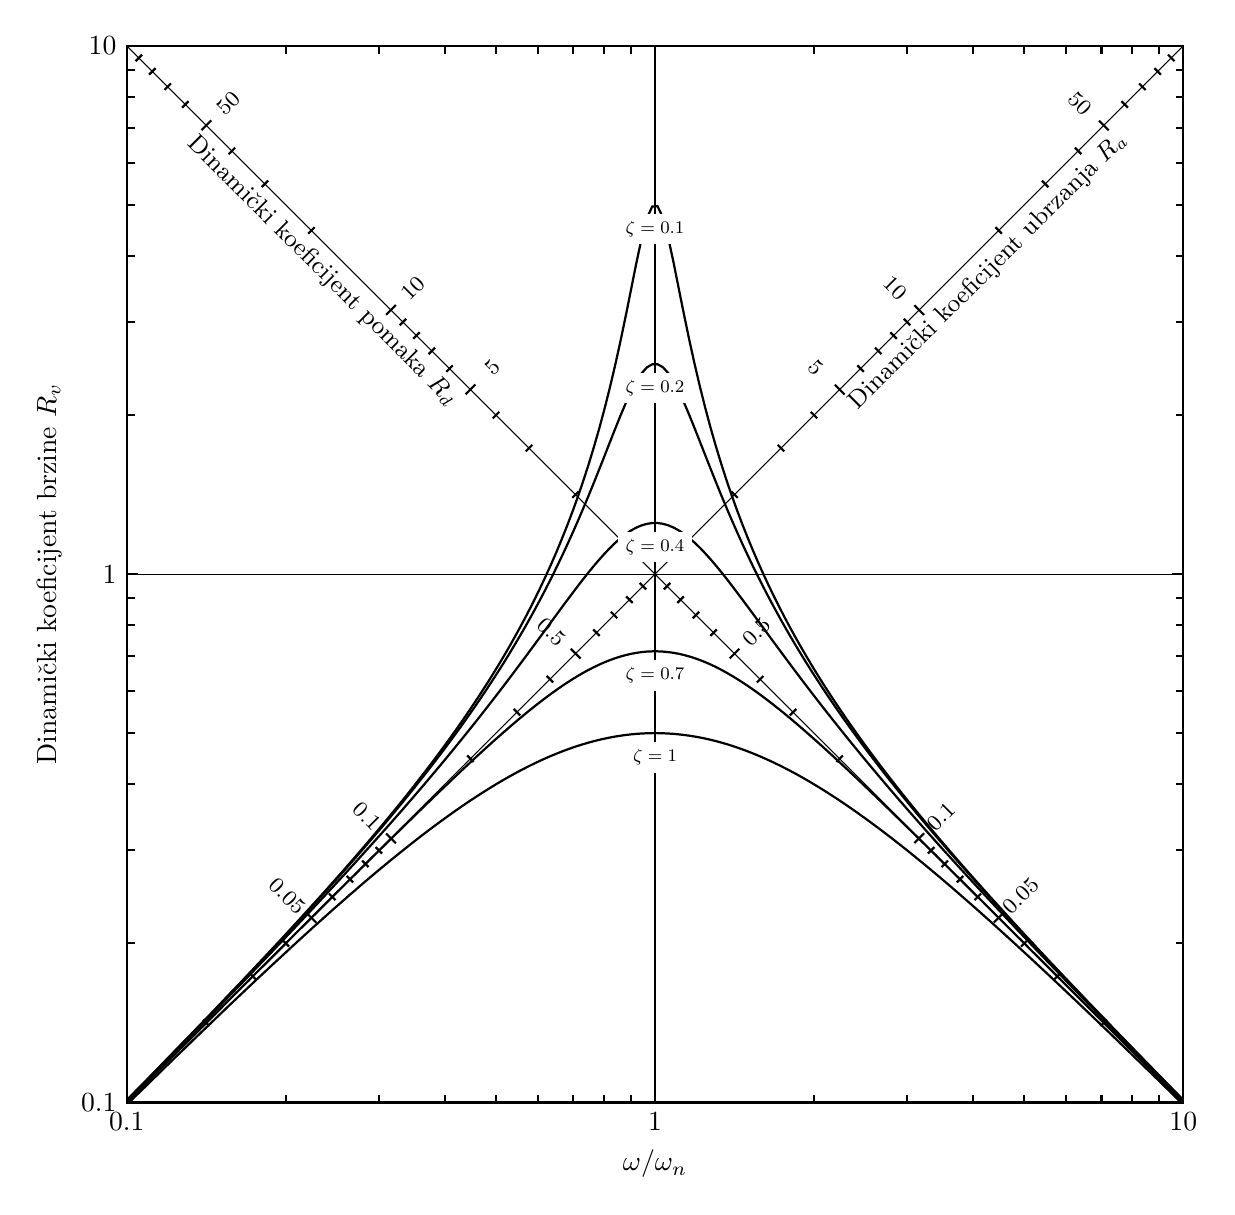
\begin{tikzpicture}%[scale=0.7]
    \begin{loglogaxis} [
        width=15cm,height=15cm,
        xmin = 0.1, xmax = 10.0,
        ymin = 0.1, ymax = 10.0,
        log ticks with fixed point,
        xlabel = $\omega/\omega_n$,
        ylabel = Dinamički koeficijent brzine $R_v$,
        ]
        \pgfplotsinvokeforeach{0.01,0.02,0.03,0.04,0.06,0.07,0.08,0.09,
                               0.2,0.3,0.4,0.6,0.7,0.8,0.9,
                               2,3,4,6,7,8,9,
                               20,30,40,60,70,80,90,100}
        {
            \draw[shift={(#1^0.5,#1^0.5)},rotate=45]
                    (1,1.02)--(1,0.98);

            \draw[shift={(1/#1^0.5,1/#1^-0.5)},rotate=135] 
                    (1,1.02)--(1,0.98);
        }

        \pgfplotsinvokeforeach{0.05,0.1,0.5,5,10,50}
        {
            \draw[shift={(#1^0.5,#1^0.5)},rotate=45]
                    (1,1.03)--(1,0.97);

            \draw[shift={(1/#1^0.5,1/#1^-0.5)},rotate=135] 
                    (1,1.03)--(1,0.97);

            %(sqrt(i)) + sqrt{i} * 0.1; sqrt{i} + sqrt{i}*0.1
            \node[shift={({#1^0.5-(#1^0.5)/10},{#1^0.5+(#1^0.5)/10})},rotate=-45]
                at(1, 1) {\footnotesize{$#1$}};

            %1/(sqrt(i)) + 1/(sqrt{i}) * 0.1; sqrt{i} + sqrt{i}*0.1
            \node[shift={({1/#1^0.5+1/#1^0.5*0.1},{#1^0.5+#1^0.5*0.1})},rotate=45]
                at(1, 1) {\footnotesize{$#1$}};
        }

        \node[rotate=45,anchor=north] at(4,4) {\small{Dinamički koeficijent ubrzanja $R_a$}};
        \node[rotate=-45,anchor=north] at(0.25,4) {\small{Dinamički koeficijent pomaka $R_d$}};
        \draw[thin](1,0.1)--(1,10);
        \draw[thin](0.1,1)--(10,1);
        \draw[thin](0.1,0.1) -- (10,10);
        \draw[thin](10.0,0.1)--(0.1,10);

        %graf
        \foreach \i in {1, 0.7, 0.4, 0.2, 0.1}
        {
            \addplot [
                domain=0.1:10.0,
                samples=200,
            ]
            {x/((1-x^2)^2 + (2*\i*x)^2)^(0.5)};
        }

        \pgfplotsinvokeforeach{1,0.7,0.4, 0.2, 0.1}
        {
            \node[rectangle,fill=white,scale=0.8] at(1,{(1-0.1)/(2*#1)})
            {\footnotesize{$\zeta=#1$}};
        }
%        \draw[thin] (1,5)--(1.5,5);
%        \draw node[rectangle, fill=white, scale=0.8] at(1.5,5){\footnotesize{$\zeta=0.1$}};
    \end{loglogaxis}
\end{tikzpicture}

    \label{fig:dva-spektar}
    \caption{Dinamički faktori pomaka, brzine i ubrzanja u logaritamskom mjerilu}
\end{figure}


